\documentclass[3p,authoryear]{elsarticle}
\journal{Annals of Nuclear Energy}

%%%%%%%%%%%%%%%%%%%%%%%%%%%%%%%%%%%%%%%%%%%%%%%%%%%%%%%%%%%%%%%%%%%%%%%%%%%%%%%%
\usepackage[charter]{mathdesign} % Type-1 Latin Modern modern
\usepackage[T1]{fontenc}         % Use T1 encoding instead of OT1
\usepackage[utf8]{inputenc}      % Use UTF8 input encoding
\usepackage{microtype}           % Improve typography
\usepackage{booktabs}            % Publication quality tables
\usepackage{amsmath}
\usepackage{amsthm}
\usepackage{float}
\usepackage{algorithm}
\usepackage{algorithmicx}
\usepackage{algpseudocode}
\usepackage{siunitx}
\usepackage{multirow}
\usepackage{upgreek}

\sisetup{list-final-separator = {, and }}

% Captions for figures and tables
\usepackage[labelfont=bf]{caption}
\captionsetup[figure]{labelsep=period, name=Fig.}
\captionsetup[table]{labelsep=newline}

\usepackage{color}
\definecolor{aneblue}{RGB}{0,128,173}
\usepackage[colorlinks,breaklinks,bookmarksnumbered,bookmarksopen]{hyperref}
\AtBeginDocument{
  \hypersetup{linkcolor=aneblue, citecolor=aneblue, urlcolor=aneblue}
}

\usepackage[capitalise,nameinlink]{cleveref}

\newtheorem{lemma}{Lemma}

\newcommand{\vect}[1]{\mathbf{#1}} % vectors and matrices

%%%%%%%%%%%%%%%%%%%%%%%%%%%%%%%%%%%%%%%%%%%%%%%%%%%%%%%%%%%%%%%%%%%%%%%%%%%%%%%%
\begin{document}

\title{Depletion capabilities in the OpenMC Monte Carlo particle transport code}

\author[anl]{Paul K. Romano\corref{cor1}}
\ead{promano@anl.gov}
\cortext[cor1]{Corresponding author. Tel.: +1 630 252 6779.}

\author[lanl]{Colin Josey}
\ead{cjosey@lanl.gov}

\author[gatech]{Andrew E. Johnson}
\ead{dasindrew@gatech.edu}

\author[tsinghua]{Jingang Liang}
\ead{jingang@tsinghua.edu.cn}

\address[anl]{Argonne National Laboratory, 9700 S. Cass Ave, Lemont, IL 60439, United States}
\address[lanl]{Los Alamos National Laboratory, P.O. Box 1663, Los Alamos, NM 87545, United States}
\address[gatech]{Georgia Institute of Technology, 770 State St NW, Atlanta, GA 30318, United States}
\address[tsinghua]{Institute of Nuclear and New Energy Technology, Tsinghua University, Beijing, China}

\begin{abstract}

\end{abstract}

\begin{keyword}
  Monte Carlo, depletion
\end{keyword}

\maketitle

%%%%%%%%%%%%%%%%%%%%%%%%%%%%%%%%%%%%%%%%%%%%%%%%%%%%%%%%%%%%%%%%%%%%%%%%%%%%%%%%
\section{Introduction}

When a material in a system is subject to irradiation over a long period of
time, nuclides within the material will transmute due to nuclear reactions and
spontaneous radioactive decay. The time-dependent process by which nuclides
transmute under irradiation is known as \emph{depletion}, \emph{burnup}, or
\emph{transmutation}. Modeling this process plays an important role in the
design and licensing of nuclear reactors~\citep{betzler2019ned}. Consequently,
many codes have been developed that solve the underlying equations for the
change in material compositions over time.

When modeling nuclear reactors, depletion is inherently linked with solving the
neutron transport equation. Nuclear reaction rates, which determine the rate at
which nuclides are transmuted, must be provided from a transport code.
Conversely, the change in material composition directly affects the solution of
the transport equation. As will be shown in \cref{sec:methods}, this results in
a non-linear coupling between transport and depletion. The implication is that
depletion codes are rarely used in isolation---normally, they are directly
coupled with a neutron transport code.

With continued advances in computing, Monte Carlo (MC) particle transport
simulations are now widely used in reactor design and analysis in a variety of
roles. The earliest efforts to couple MC particle transport with depletion date
back to the 1990s~\citep{moore1995inel,trellue1998lanl}. These early efforts
involved taking existing MC and depletion codes, such as
MCNP~\citep{goorley2012nt} and ORIGEN~\citep{croff1983nt}, and putting a
``wrapper'' around them that orchestrated the transfer of solutions from one
code to the other. Thus, the actual transport/depletion codes themselves
required no source code changes. In the last decade, many MC code developers
have chosen to directly include a depletion solver as a first-rate feature,
including MCNPX~\citep{waters2007aip} (which has since been merged into
MCNP6~\citep{goorley2012nt}), Serpent~\citep{leppanen2015ane}, and
MC21~\citep{griesheimer2015ane}.

In the present work, we describe a new depletion solver in
OpenMC~\citep{romano2015ane1}, an open source, community-developed MC particle
transport code. To date, OpenMC has not had a built-in depletion solver. This
has led to numerous efforts in the community toward developing coupled
transport-depletion calculations with OpenMC~\citep{gul2017ane,
lanversin2017icone, lanversin2019phd, liu2019nst, zhuang2020pne, zhao2020ned,
zhao2020cpc, zhang2020ane}. While these efforts have proven the viability of
performing such coupled calculations with OpenMC, none of them has resulted in a
validated, openly-available, and generalized capability that OpenMC users can
take advantage of. The capability that is described herein is part of the OpenMC
project and can be found in version 0.11~\citep{openmc-0110} of the code or
later.

The paper is organized as follows. In \cref{sec:methods}, we describe the
methods and algorithms used to solve the depletion equations, the implementation
within OpenMC, and how nuclear data is used to create depletion chains. Then, in
\cref{sec:results}, we present results on two problems that demonstrate the
accuracy of OpenMC when compared to Serpent~\citep{leppanen2015ane}. In
\cref{sec:conclusions}, we summarize the findings, discuss limitations, and
provide commentary on future avenues of inquiry that may be promising.

%%%%%%%%%%%%%%%%%%%%%%%%%%%%%%%%%%%%%%%%%%%%%%%%%%%%%%%%%%%%%%%%%%%%%%%%%%%%%%%%
\section{Methodology}
\label{sec:methods}

The equation that governs the transmutation of nuclides by nuclear reactions and
radioactive decay inside of an irradiated environment can be written as
\begin{equation}
  \label{eq:depletion}
  \begin{split}
  \frac{dN_i(t)}{dt} = &\sum\limits_j \left [ f_{j \rightarrow i}
  \int_0^\infty dE \; \sigma_j (E, t) \phi(E,t) + \lambda_{j\rightarrow i}
  \right ] N_j(t) \\ &- \left [\int_0^\infty dE \; \sigma_i (E,t) \phi(E,t) +
  \sum\limits_j \lambda_{i\rightarrow j} \right ] N_i(t), \quad i=1,\dots,n
  \end{split}
\end{equation}
where
\begin{equation*}
  \begin{split}
  N_i(t) &\equiv \text{density of nuclide $i$ at time $t$} \\
  \sigma_i(E,t) &\equiv \text{transmutation cross section for nuclide $i$ at energy $E$ and time $t$} \\
  \phi(E,t) &\equiv \text{neutron flux at energy $E$ and time $t$} \\
  f_{j \rightarrow i} &\equiv \text{fraction of transmutation reactions in nuclide $j$ that produce nuclide $i$} \\
  \lambda_{j \rightarrow i} &\equiv \text{decay constant for decay modes in nuclide $j$ that produce nuclide $i$} \\
  n &\equiv \text{total number of nuclides.}
  \end{split}
\end{equation*}
Note that we have not included the spatial dependence of the flux or cross
sections. For \cref{eq:depletion} to be accurate, the spatial variation of the
reaction rates over the region which is being depleted should be small. For a
reactor model, this may entail using a unique material in each fuel pin that is
depleted separately. Ultimately, the user is responsible for deciding what level
of spatial discretization is adequate for the problem at hand.

\Cref{eq:depletion} simply states that the rate of change of $N_i$ is equal to
the production rate minus the loss rate. Because the equation for $N_i$ depends
on the density of other nuclides, $\{N_j \,|\, j \ne i\}$, \cref{eq:depletion}
represents a system of first-order ordinary differential equations (ODEs). To
form a proper initial value problem, the nuclide densities at time 0 must be
specified:
\begin{equation}
    N_i(0) = N_{i,0}.
\end{equation}
These equations can be written more compactly in matrix notation as
\begin{equation}
  \label{eq:depletion-matrix-t}
  \frac{d\vect{n}}{dt} = \vect{A}(\vect{n},t)\vect{n}, \quad \vect{n}(0) =
  \vect{n}_0
\end{equation}
where
\begin{equation}
  \vect{n} = \begin{pmatrix} N_1 \\ N_2 \\ \vdots \\ N_n \end{pmatrix}, \quad
  \vect{n}_0 = \begin{pmatrix} N_{1,0} \\ N_{2,0} \\ \vdots \\ N_{n,0} \end{pmatrix}
\end{equation}
and $\vect{A}(\vect{n},t) \in \mathbb{R}^{n\times n}$ is the burnup matrix
containing the decay and transmutation coefficients. Note that the burnup matrix
depends on $\vect{n}$ because the solution to the transport equation depends
on the nuclide densities, thereby making \cref{eq:depletion-matrix-t} nonlinear.

Although the neutron transport equation is time-dependent, the timescale over
which material compositions change is sufficiently long such that the transport
equation can be solved as a time-independent equation. Without loss of
generality, let us write the burnup matrix solely as a function of $\vect{n}$
so that \cref{eq:depletion-matrix-t} becomes
\begin{equation}
  \label{eq:depletion-matrix}
  \frac{d\vect{n}}{dt} = \vect{A}(\vect{n})\vect{n}, \quad \vect{n}(0) =
  \vect{n}_0.
\end{equation}
This better reflects the fact that the time, $t$, is generally not an input to
the transport equation, and hence the burnup matrix is uniquely determined by
the value of $\vect{n}$.

The principle difficulty of solving \cref{eq:depletion-matrix} is the fact that
the elements of $\vect{A}$ are not constant with respect to time. If
$\vect{A}$ is constant, \cref{eq:depletion-matrix} admits a closed-form
solution,
\begin{equation}
  \label{eq:constant-A}
  \vect{n}(t) = \exp \left (\vect{A} t \right ) \vect{n}_0.
\end{equation}
The exponential of a matrix $\vect{X}$ is defined by the power series
expansion
\begin{equation}
  \exp(\vect{X}) = \sum\limits_{k=0}^\infty \frac{\vect{X}^k}{k!}
\end{equation}
where $\vect{X}^0 = \vect{I}$. Solving \cref{eq:depletion-matrix} usually
involves two separate components:
\begin{enumerate}
  \item Use of a numerical method to integrate \cref{eq:depletion-matrix}
  forward in time, usually in a form that involves taking one or more matrix
  exponentials, and
  \item Evaluating the matrix exponential or, equivalently, the action of a
  matrix exponential on a vector.
\end{enumerate}
We will henceforth refer to the first component as \emph{time integration}. Let
us now consider how each of these components are treated in OpenMC.

\subsection{Time Integration}
\label{sec:time_integration}

Because an analytical solution to \cref{eq:depletion-matrix} is not available,
one must resort to using a numerical method that generates approximate solutions
in discrete increments. The problem we need to solve then is: given $\vect{n}_i
\equiv \vect{n}(t_i)$, what is the value of $\vect{n}_{i+1} \equiv
\vect{n}(t_{i+1}) = \vect{n}(t_i + h)$, with $h$ being the step size? Without
loss of generality, we shall choose $t_i=0$ as it makes the presentation of
various methods simpler.

OpenMC doesn't rely on a single time integration method but instead has several
methods available that the user can choose. In the following sections, we
outline the available methods in OpenMC, several of which have not been
previously described in the literature.

\subsubsection{Predictor Method}

The simplest numerical method for solving \cref{eq:depletion-matrix} over a
timestep is known as the \emph{predictor} method. It proceeds by assuming that
$\vect{A}$ is constant over the timestep and assumes the value at the
beginning of the step. The solution then follows directly from
\cref{eq:constant-A}:
\begin{equation}
  \label{eq:predictor}
  \vect{n}_{i+1} = \exp\left(h\vect{A}(\vect{n}_i) \right) \vect{n}_i.
\end{equation}
The end-of-step composition is thus ``predicted'' by the reaction rates at the
beginning of the step. This method has the virtue of requiring a single
transport solution and a single matrix exponential per timestep but is only
first-order accurate.

\subsubsection{predictor--Corrector Methods}

A series of \emph{predictor--corrector} methods that use multiple stages offer
improved accuracy over the predictor method. The simplest of these methods is
the CE/CM algorithm, which is the default algorithm used in
MCNP6~\citep{fensin2006tans}. In this method, $\vect{A}$ is evaluated at the
beginning of the step and used to deplete the composition over half the step.
Then, $\vect{A}$ is reevaluated using the predicted middle-of-step composition
and used to deplete over the full step. The algorithm can be expressed as
\begin{equation}
  \begin{split}
    \vect{n}_{i+1/2} &= \exp \left (\frac{h}{2}\vect{A}(\vect{n}_i) \right) \vect{n}_i \\
    \vect{n}_{i+1} &= \exp \left(h \vect{A}(\vect{n}_{i+1/2}) \right) \vect{n}_i.
  \end{split}
\end{equation}
This method requires two transport solutions and two matrix exponential solves
per timestep (twice as expensive as the predictor method) and is second-order
accurate.

More sophisticated predictor--corrector methods have been introduced by
\citet{isotalo2011ane2,isotalo2011ane3}. In the CE/LI (constant extrapolation,
linear interpolation) method, the end-of-step composition is first predicted
using $\vect{A}(\vect{n}_i)$:
\begin{equation}
  \vect{n}_{i+1}^p = \exp \left( h\vect{A}(\vect{n}_i) \right) \vect{n}_i.
\end{equation}
Then, $\vect{n}_{i+1}^p$ is used to reevaluate $\vect{A}$. An approximation of
$\vect{A}$ that depends on time is formed by linearly interpolating between
$\vect{A}(\vect{n}_i)$ and $\vect{A}\left(\vect{n}_{i+1}^p\right)$.
\Cref{eq:depletion-matrix} thus becomes
\begin{equation}
  \label{eq:linear-ode}
  \frac{d\vect{n}}{dt} = \hat{\vect{A}}(t) \vect{n}
\end{equation}
where
\begin{equation}
  \label{eq:linear-interp}
  \hat{\vect{A}}(t) = \left ( 1 - \frac{t}{h} \right) \vect{A}(\vect{n}_i) +
  \frac{t}{h} \vect{A}\left(\vect{n}_{i+1}^p \right).
\end{equation}
We see that $\hat{\vect{A}}$ no longer depends on $\vect{n}$ thereby making
\cref{eq:linear-ode} a linear nonautonomous ODE. Because $\hat{\vect{A}}$ is a
function of time, an approximation is still needed to obtain $\vect{n}_{i+1}$.
The simplest approach~\citep{isotalo2011ane2} is to average
\cref{eq:linear-interp} over the step,
\begin{equation}
  \bar{\vect{A}} = \int_0^h dt \, \hat{\vect{A}}(t) = \frac{\vect{A}(\vect{n}_i)
  + \vect{A}(\vect{n}_{i+1}^p)}{2},
\end{equation}
and then use $\bar{\vect{A}}$ to deplete over the full step:
\begin{equation}
  \vect{n}_{i+1} = \exp \left ( h \bar{\vect{A}} \right ) \vect{n}_i.
\end{equation}
\citet{isotalo2011ane3} suggested an improvement over this approach wherein
$\hat{\vect{A}}$ is averaged over substeps instead of the entire interval. That
is, if we divide the timestep into $m$ substeps, the solution is given by
\begin{equation}
  \begin{split}
    \label{eq:celi-substeps}
    \vect{A}_s &= \int_{(s-1)h/m}^{sh/m} dt \; \hat{\vect{A}}(t), \quad s=1,\dots,m \\
    \vect{n}_{i+1} &= \exp\left(\vect{A}_m \right) \exp \left(\vect{A}_{m-1}\right)
    \cdots \exp\left(\vect{A}_1\right) \vect{n}_i.
  \end{split}
\end{equation}
While using substeps is a reasonable approach for solving \cref{eq:linear-ode},
there are other methods as well. For example, some codes use a backward
differentiation formula rather than a method based on an exponential
integrator~\citep{carpenter2009mc,hykes2017mc,sublet2017nds}.

\subsubsection{Magnus expansion integrators}

Any linear approximation of \cref{eq:depletion-matrix} characterized by
$\vect{A}$ that depends only on time, such as \cref{eq:linear-ode}, has an
infinite series solution known as the Magnus expansion~\citep{blanes2009pr}.
This expansion takes the form
\begin{equation}
  \begin{split}
  \vect{n}(t) &= \exp \left( \vect{\Omega}(t) \right ) \vect{n}_0 \\
  \vect{\Omega}(t) &= \sum\limits_{k=1}^\infty \vect{\Omega}_k(t).
  \end{split}
\end{equation}
The first three terms of the expansion are given by
\begin{equation}
  \label{eq:magnus-terms}
  \begin{split}
    \vect{\Omega}_1(t) &= \int_0^t dt_1 \vect{A}(t_1) \\
    \vect{\Omega}_2(t) &= \int_0^t dt_1 \int_0^{t_1} dt_2 [\vect{A}(t_1), \vect{A}(t_2) ] \\
    \vect{\Omega}_3(t) &= \int_0^t dt_1 \int_0^{t_1} dt_2 \int_0^{t_2} dt_3
      \left ( [\vect{A}(t_1), [\vect{A}(t_2), \vect{A}(t_3)]] + [\vect{A}(t_3), [\vect{A}(t_2), \vect{A}(t_1)]] \right )
  \end{split}
\end{equation}
where $[\vect{A},\vect{B}] = \vect{A}\vect{B} - \vect{B}\vect{A}$ is a matrix
commutator. Subsequent terms can be defined through a recurrence relation.

The Magnus expansion can be used as the basis for developing numerical
integration algorithms and has been widely studied. The typical approach is to
truncate the $\vect{\Omega}$ series at an appropriate order and apply an
approximation to the multivariate integrals in \cref{eq:magnus-terms}. In
particular, OpenMC uses a fourth-order commutator-free\footnote{The integrator
is called commutator-free because it does not require computing any matrix
commutators like those that appear in \cref{eq:magnus-terms}. Other methods
based on the Magnus expansion do require computing matrix commutators, some of
which were explored by \citet{josey2017phd}.} exponential
integrator~\citep{blanes2006anm} that is derived from the Magnus expansion in
order to solve \cref{eq:linear-ode}. In this approximation, the Magnus expansion
is truncated at two terms and then expressed as the composition of two
exponentials. For a system of ODEs in the form of \cref{eq:linear-ode}, the
resulting method is
\begin{equation}
  \label{eq:compose4}
  \vect{n}_{i+1} = \exp (a_2 \vect{A}_1 + a_1 \vect{A}_2)
  \exp (a_1 \vect{A}_1 + a_2 \vect{A}_2) \vect{n}_i
\end{equation}
where $\vect{A}_1$ and $\vect{A}_2$ correspond $\hat{\vect{A}}$ evaluated at the
nodes of a two-point Gauss-Legendre quadrature over the interval $[0,h]$:
\begin{equation}
  \begin{split}
    a_1 &= \frac{1}{4} + \frac{\sqrt{3}}{6}, \; a_2 = \frac{1}{4} - \frac{\sqrt{3}}{6} \\
    c_1 &= \frac{1}{2} - \frac{\sqrt{3}}{6}, \; c_2 = \frac{1}{2} + \frac{\sqrt{3}}{6} \\
    \vect{A}_1 &= h\hat{\vect{A}}\left ( c_1 h\right ), \; \vect{A}_2 = h\hat{\vect{A}}\left ( c_2 h\right ).
  \end{split}
\end{equation}
Evaluating $\vect{A}_1$ and $\vect{A}_2$ using \cref{eq:linear-interp} and
substituting in \cref{eq:compose4}, we obtain a CE/LI method based on the
fourth-order commutator-free Magnus integrator:
\begin{equation}
  \label{eq:celi-cfq4}
  \begin{split}
  \vect{n}_{i+1}^p &= \exp \left ( h \vect{A}(\vect{n}_i ) \right ) \\
  \vect{n}_{i+1} &= \exp \left( \frac{h}{12} \vect{A}(\vect{n}_i) +
    \frac{5h}{12} \vect{A}(\vect{n}_{i+1}^p) \right)
  \exp \left( \frac{5h}{12} \vect{A}(\vect{n}_i) +
  \frac{h}{12} \vect{A}(\vect{n}_{i+1}^p) \right) \vect{n}_i.
  \end{split}
\end{equation}
\Cref{eq:celi-cfq4} requires two transport solutions and two matrix
exponentials, whereas the CE/LI method with substeps, \cref{eq:celi-substeps},
requires two transport solutions and $m$ matrix exponentials. A comparison of
these two approaches has shown that \cref{eq:celi-cfq4} achieves better accuracy
than the use of five substeps~\citep{josey2017phd}. OpenMC also includes an
integrator based on the LE/QI (linear extrapolation, quadratic interpolation)
method~\citep{isotalo2011ane2} where the integration of \cref{eq:linear-ode} (in
which case $\hat{\vect{A}}(t)$ is represented by a quadratic polynomial in $t$)
is performed using the fourth-order commutator-free Magnus integrator based on
\cref{eq:compose4}.

\subsubsection{Lie Group Integrator}

OpenMC also includes an integrator based on a commutator-free Lie group
integration method~\citep{celledoni2004fgcs}. In particular, a fourth-order
scheme called CF4 is used that is given as
\begin{equation}
  \begin{split}
    \vect{A}_1 &= h\vect{A}(\vect{n}_0) \\
    \hat{\vect{n}}_1 &= \exp \left ( \frac{\vect{A}_1}{2} \right ) \\
    \vect{A}_2 &= h\vect{A}(\hat{\vect{n}}_1) \\
    \hat{\vect{n}}_2 &= \exp \left ( \frac{\vect{A}_2}{2} \right ) \\
    \vect{A}_3 &= h \vect{A}(\hat{\vect{n}}_2) \\
    \hat{\vect{n}}_3 &= \exp \left ( -\frac{\vect{A}_1}{2}  + \vect{A}_3 \right ) \\
    \vect{A}_4 &= h\vect{A}(\hat{\vect{n}}_3) \\
    \vect{n}_{i+1} &= \exp \left ( \frac{\vect{A}_1}{4} + \frac{\vect{A}_2}{6} + \frac{\vect{A}_3}{6} - \frac{\vect{A}_4}{12} \right )
    \exp \left ( -\frac{\vect{A}_1}{12} + \frac{\vect{A}_2}{6} + \frac{\vect{A}_3}{6} - \frac{\vect{A}_4}{4} \right ) \vect{n}_i.
  \end{split}
\end{equation}
This method requires four transport solutions and five matrix exponentials per
timestep. However, because it is fourth-order, it allows large timesteps to be
used without sacrificing accuracy. For example, on a test problem based on a
3$\times$3 fuel pin array with gadolinum as a burnable absorber, the CF4 method
allowed 20 day timesteps while still achieving an accuracy of of 0.1\% on the
$^{157}$Gd number density~\citep{josey2017phd}.

\subsubsection{Extended Predictor--Corrector Methods}

One option to improve on the traditional predictor--corrector methods is to add
intermediate steps at which $\vect{A}$ is evaluated and combine them in such a
way as to reduce the error of the solution. The general method would take the
following form:
\begin{equation}
  \label{eq:epc}
  \begin{split}
    \hat{\vect{n}}_1 &= \vect{n}_i \\
    \hat{\vect{n}}_k &= \exp \left( h \sum_{j=1}^{k-1} a_{ij} \vect{A}(\hat{\vect{n}}_j) \right) \vect{n}_i \\
    \vect{n}_{i+1} &= \exp \left( h \sum_{j=1}^{s} b_{j} \vect{A}(\hat{\vect{n}}_j) \right) \vect{n}_i
  \end{split}
\end{equation}
Noting that the coefficients in \cref{eq:epc} can be arranged in a Butcher
tableau, \citet{josey2016jcp} proposed using the coefficients for the classic
fourth Runge--Kutta method:
\begin{equation}
  \begin{split}
    \vect{A}_1 &= h\vect{A}(\vect{n}_0) \\
    \hat{\vect{n}}_1 &= \exp \left ( \frac{\vect{A}_1}{2} \right ) \\
    \vect{A}_2 &= h\vect{A}(\hat{\vect{n}}_1) \\
    \hat{\vect{n}}_2 &= \exp \left ( \frac{\vect{A}_2}{2} \right ) \\
    \vect{A}_3 &= h \vect{A}(\hat{\vect{n}}_2) \\
    \hat{\vect{n}}_3 &= \exp \left ( \vect{A}_3 \right ) \\
    \vect{A}_4 &= h\vect{A}(\hat{\vect{n}}_3) \\
    \vect{n}_{i+1} &= \exp \left ( \frac{\vect{A}_1}{6} + \frac{\vect{A}_2}{3}
      + \frac{\vect{A}_3}{3} + \frac{\vect{A}_4}{6} \right ) \vect{n}_i.
  \end{split}
\end{equation}

\subsubsection{Stochastic Implicit Euler Integrators}

All of the integration methods discussed thus far are explicit methods that are
only conditionally stable. There are many well-documented cases where
oscillatory behavior and diverging solutions have been observed. To address
this, \citet{dufek2013ane} proposed an implicit-Euler-like method that is
unconditionally stable. The main idea is to replace $\vect{A}(\vect{n}_i)$ with
$\vect{A}(\vect{n}_{i+1})$ in \cref{eq:predictor}:
\begin{equation}
  \label{eq:implicit}
  \vect{n}_{i=1} = \exp \left( h\vect{A}(\vect{n}_{i+1}) \right) \vect{n}_i.
\end{equation}
This results in a non-linear equation for $\vect{n}_{i+1}$ that can't be solved
directly. However, it is possible to solve for $\vect{n}_{i+1}$ using a
fixed-point iteration. \citet{dufek2013ane} utilized a stochastic approximation
based on the Robbins-Monro algorithm~\citep{robbins1951ams} in order to
guarantee convergence of the fixed-point iteration while accounting for
stochasticity in the MC transport solver.

The major downside of an algorithm based on \cref{eq:implicit} is that, like the
predictor method, it is only first-order accurate. Implicit methods have also
been applied to higher-order
algorithms~\citep{kotlyar2014ane,kotlyar2016ane,cosgrove2020ane}, thereby
obtaining methods that are unconditionally stable and accurate with longer
timesteps. In OpenMC, stochastic implicit versions of the CE/LI and LE/QI
methods have also been implemented. The basis for the algorithm is to iterate on
$\vect{n}_{i+1}^p$ used in \cref{eq:linear-interp}, obtaining progressively
better estimates that are then used to solve \cref{eq:linear-ode}. A full
discussion of the algorithm and its performance and tradeoffs can be found in
\citep{josey2017phd}.

\subsubsection{Summary}

OpenMC does not rely on a single time integration method but rather has several
classes that implement different algorithms. Generally, there is a tradeoff
between the accuracy of the method, the computational expense, and the memory
requirements. When a MC code is used, the expense is dominated by the time
to compute the transport solution, i.e., to evaluate $\vect{A}$ for a given
$\vect{n}$. Thus, the cost of a method scales with the number of $\vect{A}$
evaluations that are performed per timestep. On the other hand, methods that
require more evaluations generally achieve higher accuracy. The predictor method
only requires one evaluation and its error converges as $\mathcal{O}(h)$. The
CE/CM method requires two evaluations and is thus twice as expensive as the
predictor method, but achieves an error of $\mathcal{O}(h^2)$. An exhaustive
description of time integration methods and their merits can be found in the
thesis of \citet{josey2017phd}.


\subsection{Matrix Exponential}

As we saw in \cref{sec:time_integration}, numerically integrating
\cref{eq:depletion-matrix} requires evaluating one or more matrix exponentials.
OpenMC uses the Chebyshev rational approximation method (CRAM), which was
introduced in a series of papers by Pusa~\citep{pusa2010nse,pusa2011nse}, to
evaluate matrix exponentials. In particular, OpenMC utilizes an incomplete
partial fraction (IPF) form~\citep{pusa2016nse} of CRAM that provides a good
balance of numerical stability and efficiency. In this representation the matrix
exponential is approximated as
\begin{equation}
    \exp(\vect{A}t) \approx \alpha_0 \prod\limits_{\ell=1}^{k/2} \left (
    \vect{I} + 2 \text{Re} \left ( \widetilde{\alpha}_\ell \left (\vect{A}t
    - \theta_\ell \vect{I} \right )^{-1} \right ) \right )
\end{equation}
where $k$ is the order of the approximation and $\alpha_0$,
$\widetilde{\alpha}_\ell$, and $\theta_\ell$ are coefficients that have been
tabulated for orders up to $k=48$. Rather than computing the full approximation
and then multiplying it by a vector, \cref{alg:cram}\footnote{The original
description of the algorithm presented by \citet{pusa2016nse} contains a typo.}
is used to incrementally apply the terms within the product. The $k$th order
approximation for CRAM requires solving $k/2$ sparse linear systems. OpenMC
relies on functionality from scipy.sparse.linalg for solving the linear system.
\begin{algorithm}[H]
  \caption{Incomplete partial fraction form of CRAM.}
  \label{alg:cram}
  \begin{algorithmic}[1]
    \State $\vect{n} \gets \vect{n_0}$
    \For{$\ell \gets 1$ \textbf{to} $k/2$}
      \State $\vect{n} \gets \vect{n} + 2\text{Re}(\widetilde{\alpha}_\ell
        (\vect{A}t - \theta_\ell)^{-1})\vect{n}$
    \EndFor
    \State $\vect{n} \gets \alpha_0 \vect{n}$
  \end{algorithmic}
\end{algorithm}

\subsection{Nuclear Data Considerations}

In principle, using CRAM for evaluating matrix exponentials is fairly simple:
construct the burnup matrix at various times and solve a set of sparse linear
systems. However, constructing the burnup matrix, $\vect{A}$, involves not only
solving the transport equation to estimate nuclear reaction rates but also a
series of choices about what data to include.

\subsubsection{Depletion Chain Generation}
\label{sec:depletion-chain}

In OpenMC, the burnup matrix is constructed based on data inside of a
\emph{depletion chain} file, which includes fundamental data gathered from ENDF
incident neutron, decay, and fission product yield sublibraries. For each
nuclide, this file includes:
\begin{itemize}
  \item What transmutation reactions are possible, their Q values, and their products;
  \item If a nuclide is not stable, what decay modes are possible, their
  branching ratios, and their products; and
  \item If a nuclide is fissionable, the fission products yields at any number
  of incident neutron energies.
\end{itemize}

Depletion chains can be automatically created in the Python API in the following
manner. First, the user supplies a list of ENDF incident neutron, decay, and
fission product yield sublibrary files. The incident neutron files are used to
determine what nuclear reactions result in transmutation and what the
corresponding Q values of the reactions are. The decay files are used to
determine the half-life and possible decay modes of nuclides that are unstable.
The fission product yield sublibraries are used to determine what fission
products are produced when a fission reaction occurs. This information is then
aggregated and written to an XML file that serves as the depletion chain file
that is used at runtime to construct a burnup matrix.

In some cases, decay or reaction products appear that do not actually exist in
the decay sublibrary files. OpenMC uses a set of heuristics to find a suitable
replacement. First, if the atomic number of the missing product is greater than
98, it is assumed that the product undergoes alpha decay. Otherwise, for a given
product, OpenMC will determine the mass number of the isotope of that element
that has the longest half-life. If the mass number of the missing product is
less than the mass number of the longest-lived isotope, it is assumed that the
nuclide will undergo a $\upbeta^+$ decay. Conversely, if the mass number is
larger than the mass number of the longest-lived isotope, it is assumed that the
nuclide will undergo a $\upbeta^-$ decay. Once the replacement nuclide has been
determined, OpenMC will check again if it exists in the decay sublibrary files.
If not, the process is repeated.

Using all incident neutron, decay, and fission product yield sublibrary files
from an ENDF-format library, such as ENDF/B-VIII.0, results in a \emph{full}
depletion chain that typically includes thousands of nuclides. Because the use
of a chain with $n$ nuclides will result in an $n\times n$ burnup matrix, there
is an incentive to reduce the number of nuclides in the depletion chain to
minimize both the size of the burnup matrix and the number of nuclides that are
tracked during a transport solve. The depletion chain class in OpenMC's Python
API includes a method for automatically reducing the size of the chain. Starting
with a set of nuclides that must be included, the method will recursively go
through all decay and reaction modes to determine what products may be produced.
Using this method on the ENDF/B-VII.1 library starting from a list of all stable
or very long lived (half-life greater than $10^{15}$ sec) nuclides reduces the
total number of nuclides in the depletion chain from 3,820 to 1,693.

In addition to the full depletion chain, a simplified depletion chain based on
the VERA depletion benchmark specification~\cite{kim2015casl} was created and
made available for users at \url{https://openmc.org}. This chain includes 223
nuclides and has adjusted branching ratios for some nuclides to preserve
accuracy of nuclide production rates. \Cref{fig:chains} shows which nuclides are
included in each of the depletion chains.
\begin{figure}
  \centering
  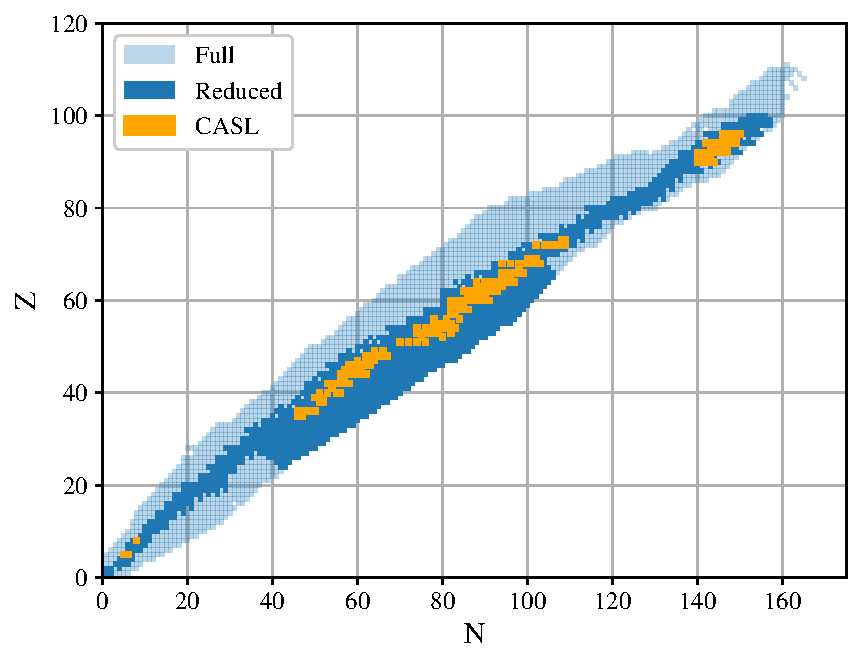
\includegraphics[width=4in]{figures/chains.pdf}
  \caption{Table of nuclides showing which nuclides are included in each of the
    depletion chains based on ENDF/B-VII.1.}
  \label{fig:chains}
\end{figure}

\subsubsection{Transmutation Reactions}

OpenMC will setup tallies in a problem based on what transmutation reactions are
available in a depletion chain file, so any arbitrary number of transmutation
reactions can be tracked. By default, the automatic depletion chain generation
described in \cref{sec:depletion-chain} will include the following transmutation
reactions: fission, (n,$\gamma$), (n,2n), (n,3n), (n,4n), (n,p), and
(n,$\alpha$). While this is suitable for fission applications, fusion
applications may require a wider set of transmutation reactions to be tracked.
Currently, reaction rates are determined by directly tallying the reaction rates
using a tracklength estimator.

\subsubsection{Capture Branching Ratios}

(n,$\gamma$) reactions may result in a product nucleus being in either the
ground state or an excited state. If the excited state is a metastable state
(having an unusually long half-life), it is important to account for this
difference during depletion. The most well-known example is capture in
$^{241}$Am, which can produce either $^{242}$Am or $^{242\text{m}}$Am. Because the
metastable state has a significantly longer half-life than the ground state, it
is important to account for the branching of the capture reaction in $^{241}$Am
to accurately predict the production of higher actinides~\citep{haeck2012nse}.
This is complicated by the fact that the branching ratio may depend on the
incident neutron energy causing capture.

OpenMC does not currently implement a method to handle energy-dependent capture
branching ratios directly. However, the depletion chain file does allow a
reaction to be listed multiple times with different branching ratios that result
in different products. Spectrum-averaged capture branching ratios have been
computed in LWR and SFR spectra and are available at
\url{https://openmc.org/depletion-chains}. Within the Python API, the class
representing a depletion chain allows branching ratios to be easily retrieved
and changed. We note that while this treatment doesn't accurately account for
the change in the capture branching ratio with increasing burnup (due to
spectral changes), these changes are generally much smaller than the differences
in capture branching ratios between nuclear data evaluations.

\subsubsection{Fission Product Yields}

Like capture branching ratios, fission product yields (FPYs) also depend on the
incident neutron energy. ENDF fission product yield sublibraries typically
include yields tabulated at two or three energies (thermal, fast, and fusion
energies). Complicating matters is the fact that while these data are specified
for a single energy, they actually represent the observed FPYs for a spectrum of
energies (characterized by a single point). For example, FPYs are often given at
\SI{0.0253}{\electronvolt}, but this actually represents the observed FPY under
a thermal neutron spectrum that contains a continuum of energies. The ENDF-6
formats manual~\citep{trkov2018bnl} recommends using linear-linear interpolation
between energy points. However, at the end of a transport solve, we typically
have a one-group or multigroup fission reaction rate---it's not clear how one
should use this information to calculate an effective FPY.

Different codes have adopted different approaches in how to handle the energy
dependence of FPYs. In ORIGEN, the average neutron energy causing fission is
calculated, and FPYs are interpolated using this average
energy~\citep{gauld2011nt}. In MCNP, the fission rate is tallied over a few
energy groups (thermal, fast, and high energy), and the energy group that
contains the majority of fissions is used to select appropriate
FPYs~\citep{fensin2008nt,fensin2011lanl}. In Serpent, a linear interpolation
factor is scored based on the neutron energy causing fission in relationship to
the energy points at which FPY are tabulated; the interpolation factor is then
used to calculate an effective FPY~\citep{kunchev2019mc}.

Rather than choose a single method, OpenMC includes three methods for treating
the energy dependence of FPYs. In the first method, FPY data corresponding to a
specific energy is manually selected. This approach may be appropriate if it is
known that neutrons in the system under consideration have a typical thermal,
fast, or fusion energy spectrum. In the second method, fission rates are tallied
above and below a specified cutoff energy. Then, thermal FPYs are used for all
fissions below the cutoff energy, and fast FPYs are used for all fissions above
the cutoff energy. In the third method, the average energy at which fission
events occur is tallied,
\begin{equation}
  \bar{E} = \frac{\int_0^\infty dE \; E \sigma_f(E)\phi(E)}{\int_0^\infty \sigma_f(E) \phi(E)},
\end{equation}
where $\sigma_f$ is the microscopic fission cross section and $\phi$ is the
neutron flux. An effective FPY is then calculated by linearly interpolating
between tabulated FPYs using the average energy. This approach is effectively
the same as that used by ORIGEN~\citep{gauld2011nt}.

\subsubsection{Power Normalization}

The reaction rates calculated by OpenMC are given in units of reactions per
source particle. For depletion, it is necessary to compute an absolute reaction
rate in reactions per second. To do so, the total observed heating in the system
is determined, and then the ratio of the system power to the observed heating is
used as a normalization factor on the reaction rates. OpenMC allows the total
heating to be determined by two different methods. In the first method, fission
reaction rates are multiplied by constant Q values in the depletion chain file
to estimate the total heating. This method is particularly useful for making
inter-code comparisons, where one must ensure that the same Q values for fission
are applied. In the second method, the actual heating rate is tallied over the
entire system (separate from the tally for transmutation reaction rates). This
method makes it possible to account for the energy dependence of the fission
energy release data as well as the fact that neutrons and photons may leak out
of the system, carrying away their energy with them. The latter effect may be
particularly important for small, leaky systems.

\subsection{Implementation}

OpenMC's core particle transport solver is written in C++ and is built as a
single executable. Most of the user-facing code, however, is written in Python.
Generally, to run OpenMC, a user writes a Python script that utilizes classes
and functions defined as part of an application programming interface (API) to
generate XML input files that are then read by the executable. On top of this,
OpenMC is also built as a shared library with a C++ API that can be called by
external programs. OpenMC's Python API includes bindings to the C++ API; this
enables a single run to be broken up into individual components. For example, a
function call from the Python bindings to the C++ API can initialize the solver
(reading inputs, loading cross sections, etc.) without actually performing a
simulation. A separate function call can run the transport simulation. Further
function calls allow a power user to obtain information about tally results
directly in memory from the C++ API.

OpenMC's depletion capability is implemented entirely in Python as the
\texttt{openmc.deplete} module. This module relies on the Python bindings to the
C++ API to initialize OpenMC, create tallies necessary for depletion, run
transport simulations, and obtain tally results. This approach has two primary
advantages. First, the time necessary to load cross sections is amortized
because it only has to be performed once, as opposed to once per transport
simulation. Second, using the Python bindings to the C++ API allows results to
be read directly in memory rather than using filesystem I/O, which helps to
minimizing overhead, particularly for large simulations.

The \texttt{openmc.deplete} module is designed with three key abstract classes
that represent the major components of the depletion solver. Each of the
abstract classes themselves defines an interface, that is, a set of methods that
a subclass must implement. First, the abstract \texttt{TransportOperator} class
represents a particle transport solver. Subclasses of \texttt{TransportOperator}
are required to implement a method that takes a list of nuclide densities to be
used in the problem and a system power and returns the $k$-eigenvalue and the
reaction rates resulting from the transport operator. Currently, there is a
single subclass of \texttt{TransportOperator} that interfaces with the Python
bindings to OpenMC's C++ API to call a tranport solve and obtain reaction rates.
Once reaction rates are obtained, a separate depletion chain class (that is not
abstract) uses them to construct the burnup matrix, $\vect{A}$, based on the
data present in the depletion chain.

The abstract \texttt{DepSystemSolver} class represents a solver for
\cref{eq:depletion-matrix} when $\vect{A}$ is constant (a solver that can
evaluate \cref{eq:constant-A}). Subclasses of \texttt{DepSystemSolver} are
required to implement a method that takes the burnup matrix $\vect{A}$, an
initial density vector $\vect{n}_0$, and a timestep size, and returns the
resulting nuclide densities at the end of the step. The only subclass of
\texttt{DepSystemSolver} at present is \texttt{IPFCramSolver}, which implements
the IPF form of CRAM to evaluate \cref{eq:constant-A}. Because the CRAM method
requires solving multiple sparse linear systems, this class relies on the
third-party \texttt{scipy.sparse} package~\cite{virtanen2020nm} for performing a
sparse linear solve.

The abstract \texttt{Integrator} class represents a time integration method.
This class effectively orchestrates the coupled transport-depletion simulation.
Subclasses of \texttt{Integrator} are required to implement a method that takes
an initial vector of nuclide densities, reaction rates returned from an
operator, a time interval, and a power, and returns the resulting nuclide
densities at the end of the step. Thus, \texttt{Integrator} utilizes
\texttt{TransportOperator} in order to obtain reaction rates given $\vect{n}$,
and once the burnup matrix is constructed, it utilizes \texttt{DepSystemSolver}
to deplete with a constant $\vect{A}$ as many times as is necessary. One example
of a subclass of \texttt{Integrator} is \texttt{CECMIntegrator}, which
implements the CE/CM method.

The depletion system in OpenMC is designed to be modular. Although the only
transport operator that is implemented is the OpenMC transport solver itself,
the rest of the infrastructure (time integration methods, CRAM solver) does not
rely on anything specific to OpenMC's transport solver, so one could in
principle implement a class that utilizes a different transport solver (whether
that be another Monte Carlo code or a deterministic code). Similarly, although
\texttt{IPFCramSolver} is the only depletion system solver implemented, one
could replace it with a different solver, for example, a solver based on
backward differentiation formulas.

Lastly, we note that when multiple depletable materials are present in a problem
(thereby requiring multiple independent solutions of
\cref{eq:depletion-matrix}), the work is fully parallelized over the available
processes/threads. The third-party \texttt{mpi4py} Python package is used to
distribute the material compositions among the participating MPI processes.
Then, within each process, Python's \texttt{multiprocessing} standard-library
module is used to distribute materials among threads within a single MPI
process. This matches the distributed- and shared-memory parallelization scheme
used in OpenMC's transport solver, which relies on MPI and OpenMP.

%%%%%%%%%%%%%%%%%%%%%%%%%%%%%%%%%%%%%%%%%%%%%%%%%%%%%%%%%%%%%%%%%%%%%%%%%%%%%%%%
\section{Results}
\label{sec:results}

\subsection{Data Preparation}

Using ENDF/B-VII.1 files from MCNP distribution. However, for light water
$S(\alpha,\beta)$, Serpent is not capable of handling continuous format, so the
file from ENDF/B-VII.0 was used. The evaluation didn't change between VII.0 and
VII.1, but the processing was different. For Serpent, decay and neutron fission
yield sublibraries are concatenated.

\subsection{PWR Pincell}

\subsection{SFR Assembly}


%%%%%%%%%%%%%%%%%%%%%%%%%%%%%%%%%%%%%%%%%%%%%%%%%%%%%%%%%%%%%%%%%%%%%%%%%%%%%%%%
\section{Conclusions}
\label{sec:conclusions}

%%%%%%%%%%%%%%%%%%%%%%%%%%%%%%%%%%%%%%%%%%%%%%%%%%%%%%%%%%%%%%%%%%%%%%%%%%%%%%%%
\section*{Acknowledgments}

This research was supported by the Exascale Computing Project (17-SC-20-SC), a
collaborative effort of the U.S. Department of Energy Office of Science and the
National Nuclear Security Administration. The submitted manuscript has been
created by UChicago Argonne, LLC, operator of Argonne National Laboratory under
contract DE-AC02-06CH11357.

%%%%%%%%%%%%%%%%%%%%%%%%%%%%%%%%%%%%%%%%%%%%%%%%%%%%%%%%%%%%%%%%%%%%%%%%%%%%%%%%
%\section*{References}

\bibliographystyle{elsarticle-harv}
\bibliography{references}

\clearpage
\vspace*{\fill}
\noindent\fbox{%
  \parbox{\textwidth}{%
    The submitted manuscript has been created by UChicago Argonne, LLC, Operator
    of Argonne \mbox{National} Laboratory (``Argonne'').  Argonne, a
    U.S. Department of Energy Office of Science laboratory, is operated
    under Contract No. \mbox{DE-AC02-06CH11357}.  The U.S. Government retains for
    itself, and others acting on its behalf, a paid-up nonexclusive, irrevocable
    worldwide license in said article to reproduce, prepare derivative works,
    distribute copies to the public, and perform publicly and display publicly,
    by or on behalf of the Government. The Department of Energy will provide
    public access to these results of federally sponsored research in accordance
    with the DOE Public Access
    Plan. \url{http://energy.gov/downloads/doe-public-access-plan.}
  }%
}
\vspace*{\fill}

\end{document}
